\documentclass[12pt]{report}
\usepackage{amsmath}
\usepackage[utf8]{inputenc}
\usepackage[T1]{fontenc}
\usepackage[a4paper,left=2cm,right=2cm,top=3cm,bottom=3cm]{geometry}
\usepackage[main=french]{babel}
\usepackage{lmodern}
\usepackage{graphicx}
\usepackage{float}
\usepackage{textcomp}
\usepackage{cases}
\usepackage{amsfonts,amssymb}
%\usepackage{amsmath}
\usepackage{subcaption}
\usepackage{caption}
\usepackage{todonotes}
%\usepackage{algorithm2e}
\usepackage[linesnumbered]{algorithm2e}
\RestyleAlgo{ruled}


\usepackage{float}
\usepackage{listings}

%\usepackage{amsmath}

\setlength{\parindent}{0.5cm}
\setlength{\parskip}{1ex plus 0.5ex minus 0.2ex}
\newcommand{\hsp}{\hspace{20pt}}
\newcommand{\HRule}{\rule{\linewidth}{0.5mm}}
\renewcommand{\thesection}{\arabic{section}}
\newcommand{\todoNC}[1]{\todo[inline,color = red!40]{NC : #1}}
\newcommand{\todoSD}[1]{\todo[inline,color = blue!40]{SD : #1}}
\newcommand{\todoKD}[1]{\todo[inline,color = green!40]{KD : #1}}

\newcommand{\A}{\mathbf{A}}
\newcommand{\E}{\mathbf{E}}
\newcommand{\D}{\mathbf{D}}
\newcommand{\F}{\mathbf{F}}

\newcommand{\M}{\mathbf{M}}
\newcommand{\N}{\mathbf{N}}

\newcommand{\I}{\mathbf{I}}
\newcommand{\G}{\mathbf{G}}
\newcommand{\B}{\mathbf{B}}

\newcommand{\U}{\mathbf{U}}
\newcommand{\LL}{\mathbf{L}}



\newcommand{\psh}[2]{\ensuremath{\langle #1|#2\rangle}\xspace}

\definecolor{codegreen}{rgb}{0,0.6,0}
\definecolor{codegray}{rgb}{0.5,0.5,0.5}
\definecolor{codepurple}{rgb}{0.58,0,0.82}
\definecolor{backcolour}{rgb}{0.95,0.95,0.92}
\lstdefinestyle{mystyle}{
    backgroundcolor=\color{backcolour},   
    commentstyle=\color{codegreen},
    keywordstyle=\color{magenta},
    numberstyle=\tiny\color{codegray},
    stringstyle=\color{codepurple},
    basicstyle=\ttfamily\footnotesize,
    breakatwhitespace=false,         
    breaklines=true,                 
    captionpos=b,                    
    keepspaces=true,                 
    numbers=left,                    
    numbersep=5pt,                  
    showspaces=false,                
    showstringspaces=false,
    showtabs=false,                  
    tabsize=2
}
\lstset{style=mystyle}

\usepackage[utf8]{inputenc}
\addtocounter{tocdepth}{3}
\setcounter{secnumdepth}{3}

\begin{document}

\begin{titlepage}
  \begin{sffamily}
  \begin{center}

    % Upper part of the page. The '~' is needed because \\
    % only works if a paragraph has started.
    %\begin{tabular}{cc}
       % \includegraphics[scale=0.5]{Logo_ENS_Paris_Saclay_Transparent.png}
        %\includegraphics[scale=0.15]{logo_DGM.jpg}\\
    %\end{tabular}\\[1cm]

    \textsc{\Large  }\\[0.5cm]
    \textsc{\Large CALCUL NUMERIQUE}\\[1.3cm]

    % Title
    \HRule \\[0.4cm]
    { \huge TP4 : Exploitation des structures et calcul creux \bfseries \\[0.4cm] }
    \HRule \\[1cm]

    % Author and supervisor
    \begin{minipage}{0.5\textwidth}
      \begin{flushleft} \large
        \emph{Auteurs : }\\

        M. Sébastien \textsc{Dubois}\\

      \end{flushleft}
    \end{minipage}
    \begin{minipage}{0.4\textwidth}
      \begin{flushright} \large
        \emph{Professeur: }\\
        T \textsc{Dufaud}

      \end{flushright}
    \end{minipage}

    \vfill
    \vspace{1cm}
    %\includegraphics[scale=0.2]{Couverture.jpg}
    
    
    % Bottom of the page
    {\large 17 Décembre 2021}
    \end{center}
\end{sffamily}
\end{titlepage}

\newpage
\tableofcontents

\newpage



\section{Introduction}

La résolution de systèmes linéaires dont l'application est très courante dans de nombreux problèmes mathématiques est, selon son paradigme direct, très couteux du fait d'une complexité algorithmique d'ordre $\mathcal{O}(n^3)$ sur les méthodes naives. Cependant, il est possible d'améliorer la convergence en utilisant des écritures par blocs, mais sans pouvoir réduire suffisament l'ordre de la complexité. De plus, il est difficile de paralleliser efficacement et de façon générale les résolutions directes. Il existe deux axes d'amélioration. La première stratégie consiste à exploiter le caractère creux des matrices. On rappelle que de nombreux problèmes mathématiques peuvent s'écrire sous la forme d'un système linéaire $\A x = b$ creux. Les approches CSR et bandes au sein des routines de calcul CBLAS sont étudiées. La seconde stratégie consiste à utiliser des approches d'approximation de solution par méthode itérative. Cela permet, en outre, de réduire la complexité algorithmique tout en gagnant en flexibilité d'utilisation - lorsque la précision machine n'est pas absolument nécéssaire. Il est ensuite possible de coupler les deux approches simultanément en mettant en place des résolutions itératives exploitant le caractère creux de la matrice du problème. \\
Ces stratégies seront mises en place au sein d'un code pré-écrit en \texttt{C} et au sein de \textsc{Matlab}/ \textsc{Scilab}.
\newpage 
L'ensemble des codes est disponible sur \textsc{github} suivant le lien\\
 \ref{}{https://github.com/sbstndbs/differences\_finies}.
\newpage

\section{TP4 : Exploitation de certaines propriétés des matrices dans la résolution linéaire}
\subsection{Exercice 1 : Factorisation $\mathbf{LD}\mathbf{L}^T$ pour $\mathbf{A}$ symétrique}

\textbf{Théorème}

\textbf{Si} $\mathbf{A} \in \mathbb{R}^{(n\times n )}$ est symétrique, et $\mathbf{A}(1:k, 1:k)$ inversible, \textbf{alors} $\exists ! \mathbf{L} \in ULT(\mathbb{R})^{(n \times n)}, ~ \exists ! \mathbf{D} \in Diag(\mathbb{R})^{(n \times n)} ~/~ \mathbf{A}= \mathbf{L} \mathbf{D} \mathbf{L}^T$

\textit{Note : $ULT$ signifie l'ensemble des matrices Unit Lower Triangular. Unit signifie que les termes diagonaux sont unitaires.}

\textbf{Démonstration}

Existance :
On rappelle l'existance de la décomposition $\mathbf{A} = \mathbf{L} \mathbf{U}$.
Par symetrie de $\mathbf{A}$, $\mathbf{A} = \mathbf{A}^T$. Ainsi, $\mathbf{L}\mathbf{U} =\mathbf{U}^T\mathbf{L}^T$.
Ainsi, 
\begin{equation}
\mathbf{A} = \mathbf{L} \mathbf{U} \underbrace{\Longrightarrow}_{\mathbf{A} = \mathbf{A}^T} \mathbf{L}^{-1} \mathbf{A} \mathbf{L}^{-T} = \underbrace{\mathbf{L}^{-1} \mathbf{L} \mathbf{U} \mathbf{L}^{-T}}_{symetrique} =  \underbrace{\mathbf{U} \mathbf{L}^{-T}}_{triangulaire ~superieure}
\end{equation}
L'application  de la transposition sur le terme de gauche nous permet de remarquer la symétrie de $ \mathbf{L}^{-1} \mathbf{L} \mathbf{U} \mathbf{L}^{-T}$ :
\begin{equation}
\left(\mathbf{L}^{-1} \mathbf{L} \mathbf{U} \mathbf{L}^{-T}\right)^T = \mathbf{L}^{-1} \mathbf{L} \mathbf{U} \mathbf{L}^{-T} \Longrightarrow \underbrace{\mathbf{U} \mathbf{L}^{-T}}_{triangulaire ~ superieure} = \underbrace{\left(\mathbf{U} \mathbf{L}^{-T}\right)^T}_{triangulaire ~ inferieure}
\end{equation}
Ainsi, $\mathbf{U} \mathbf{L}^{-T}$ est \textbf{diagonale} car à la fois \textbf{triangulaire supérieure et inférieure}.
En \textbf{conclusion}, $\mathbf{A} = \mathbf{L} \mathbf{U} = \mathbf{L} \underbrace{\mathbf{D}}_{\mathbf{U} \mathbf{L}^{-T}} \mathbf{L}^{T}$.

Unicité :
Par unicité de la décomposition $\mathbf{A} = \mathbf{L} \mathbf{U}$, la décompsition $\mathbf{A}= \mathbf{L} \mathbf{D} \mathbf{L}^T$ est unique (trivial : on rappelle que $\mathbf{L}$ est ULT).

Comment déterminer un algorithme ?

On cherche une expression de $d_j$ :
\begin{equation}
a_{jj} = \mathbf{L}(j, 1:j)^T . \begin{bmatrix}
d_1 l_{j,1} \\
\vdots \\
d_{j-1} l_{j,j-1} \\
d_{j}\\
\end{bmatrix} = d_j + \sum_{k=1}^{j-1} d_k l_{j,k}^2
\end{equation}
Cela permet de déterminer directement les $d_j$ suivant :
\begin{equation}
d_j = a_{jj} - \sum_{k=1}^{j-1} d_k l_{j,k}^2
\end{equation}


Une écriture permet d'obtenir

\begin{equation}
A(j+1:n,j) = L(j+1:n, 1:j-1) v(1:j-1) + d_j L(j+1:n, j)
\end{equation}

\begin{equation}
L(j+1:n, j) = \frac{1}{d_j} \left(  A(j+1:n, j) - L(j+1:n, 1:j-1) v(1:j-1) \right)
\end{equation}


Voici une proposition de l'algorithme $LDL^T$ :

\begin{algorithm}[H]
\caption{Factorisation LDLT}\label{alg:two}
\For{$j = [1:n]$}{
	$\mathbf{L}(j,j) = 1$ \;
	 \For{$i = [1:j-1]$}{
		$v_i = \mathbf{L}(j,i) \times d_i$ \;
	}
	$d_j = \mathbf{A}(j,j) - \mathbf{L}(j, 1:j-1) v(1:j-1)$  \;
	$\mathbf{L}(j+1:n, j) = \frac{1}{d_j}\left( A(j+1:n, j)  - \mathbf{L}(j+1:n, 1:j-1) v(1:j-1) \right) $  \;
}
\end{algorithm}


Une fois la factorisation obtenue, il suffit d'effectuer deux fois l'algorithme de descente et de remontée. En effet :

\begin{equation}
\mathbf{A}x = b ~\underbrace{\Longleftarrow}_{b} ~\mathbf{L} z = b~ \underbrace{\Longleftarrow}_{z} ~\mathbf{D} y = z~ \underbrace{\Longleftarrow}_{y} ~\mathbf{L}^T x = y
\end{equation}


\textit{Cependant, cette technique nécéssite une allocation d'une matrice $\mathbf{L}$. Cependant, on pourrait très bien écraser les valeurs dans $\mathbf{A}$ puisque les étapes successives ne nécéssitent plus les termes écrasés.}

Voici la réécriture de l'algorithme :

\begin{algorithm}[H]
\caption{Factorisation LDLT en place}\label{alg:two}
\For{$j = [1:n]$}{
	 \For{$i = [1:j-1]$}{
		$v_i = \mathbf{A}(j,i) \times \mathbf{A}(i,i)$ \;
	}
	$d_j = \mathbf{A}(j,j) - \mathbf{A}(j, 1:j-1) v(1:j-1)$  \;
	$\mathbf{A}(j+1:n, j) = \frac{1}{\mathbf{A}_{j,j}}\left( A(j+1:n, j)  - \mathbf{A}(j+1:n, 1:j-1) v(1:j-1) \right) $  \;
}
\end{algorithm}


Mon implémentation utilisant le \textit{slicing} sur \textsc{Matlab} est :

\begin{figure}[H]
\begin{minipage}{0.5\textwidth}
\begin{lstlisting}[language=Matlab, caption=Factorisation LDLT d'une matrice symmétrique réelle]
function [L,D] = choleskyb(A)
[n1, n2] = size(A); 
L = eye(n1,n1);
D = zeros(n1,n1);
v = zeros(n1,1);
for j = [1:n1]
    for i = [1:j-1]
        v(i) = L(j,i) * D(i,i) ; 
    end
    D(j,j)=A(j,j)-L(j,1:j-1)*v(1:j-1);

    L(j+1:n1,j)=(1/D(j,j))*
		(A(j+1:n1,j)-L(j+1:n1,1:j-1)*v(1:j-1)); 
end
\end{lstlisting}
\end{minipage}
\begin{minipage}{0.499\textwidth}
\begin{lstlisting}[language=Matlab, caption=Factorisation LDLT en place d'une matrice symmétrique réelle]
function [A] = choleskybp(A)
[n1, n2] = size(A); 


v = zeros(n1,1);
for j = [1:n1]
    for i = [1:j-1]
        v(i) = A(j,i) * A(i,i) ; 
    end
    A(j,j)=A(j,j)-A(j,1:j-1)*v(1:j-1);

    A(j+1:n1,j) = (1/A(j,j))*
		(A(j+1:n1,j)-A(j+1:n1,1:j-1)*v(1:j-1)); 
end
\end{lstlisting}
\end{minipage}
\end{figure}

L'algorithme exécute trois boucles \texttt{for} imbriquées. Le slicing masque deux boucles imbriquées, notamment par l'intermédiaire d'un produit matrice-vecteur \texttt{A(j+1:n1,1:j-1)*v(1:j-1)} de complexité $C_{mv}^{\infty} = \mathcal{O}(n^2)$ - à un coefficient multiplicateur près. La complexité asymptotique de l'algorithme entier est alors $C_{LDLT}^{\infty} = \mathcal{O}(n^3)$, similaire aux factorisations $\mathbf{LU}$. Cependant, le coefficient multiplicateur est supérieure dans ce dernier cas. Il est difficile de tenir compte de la constante pour juger de quel algorithme sera le plus efficace tant que les opérations élémentaires ne sont pas pondérées par le coût réel associé à son exécution CPU et de l'impact de la structure de données. Cependant, il y a deux fois moins de données à traiter dans le cas de la factorisation $\mathbf{LDL}^T$. 

Le cout mémoire associé à l'algorithme est de $M^{LDLT} = \frac{n \times (n+1)}{2}$ contre $M^{LU} = \frac{n \times (n+1)}{1}$.

Voici les résultats de l'exécution de l'algorithme pour une petite matrice symmétrique :

\begin{lstlisting}[language=Matlab, caption=Résultat des algorithmes de factorisation LDLT]
A_sym
    12    12    12    11
    12     4     8     1
    12     8     6    15
    11     1    15    14
L
    1.0000         0         0         0
    1.0000    1.0000         0         0
    1.0000    0.5000    1.0000         0
    0.9167    1.2500   -2.2500    1.0000
D
   12.0000         0         0         0
         0   -8.0000         0         0
         0         0   -4.0000         0
         0         0         0   36.6667
A en place
   12.0000   12.0000   12.0000   11.0000
    1.0000   -8.0000    8.0000    1.0000
    1.0000    0.5000   -4.0000   15.0000
    0.9167    1.2500   -2.2500   36.6667
L*D*LT
   12.0000   12.0000   12.0000   11.0000
   12.0000    4.0000    8.0000    1.0000
   12.0000    8.0000    6.0000   15.0000
   11.0000    1.0000   15.0000   14.0000
\end{lstlisting}
Sur la matrice $\mathbf{A}$ donnée, le résultat de la factorisation  fonctionne correctement dans les deux variantes. Il faut bien-sûr utiliser un algorithme de descente et de remontée spécifique lorsqu'est utilisé la factorisation en-place qui ne stocke pas explicitement les valeurs unitaires des diagonales de $\mathbf{L}$. L'algorithme fonctionne aussi sur des valeurs réelles tant que $\mathbf{A}$ est inversible non nécéssairement définie positive, et  sur des matrices plus grandes. 
En effet, le fait d'utiliser une factorisation $\mathbf{A} = \mathbf{LDL}^T$ et non  $\mathbf{A} = \mathbf{LL}^T$ permet d'utiliser des matrices non définies positives, c'est-à-dire des matrices $\mathbf{A} / \exists x \in \mathbb{R}^n, x^T\mathbf{A}x \le 0$. Par exemple, la matrice $-\mathbf{I}_2$ est factorisable selon $-\mathbf{I}_2 =\underbrace{ \mathbf{I}_2}_{\mathbf{L}} \underbrace{\left(- \mathbf{I}_2\right)}_{\mathbf{D}} \underbrace{\mathbf{I}_2}_{\mathbf{L}^T} $ mais il est impossible de déterminer une matrice triangulaire inférieure réelle $\mathbf{L}$ non \textit{ULD} telle que $-\mathbf{I}_2 = \mathbf{L} \mathbf{L}^T$. La factorisation codée fonctionne bien sur cet exemple d'identité, et retourne des valeurs infinies ou indéfinies dans le cas d'une matrice symmétrique non inversible, ce qui est attendu.
 
Voici ci-dessous les temps de calculs associées à la méthode. La méthode de mesure utilise des boucles repettant les execututions des algorithmes de sorte à mesurer une quantité mesurable par les fonctions \texttt{tic() toc()}.
\begin{figure}[H]
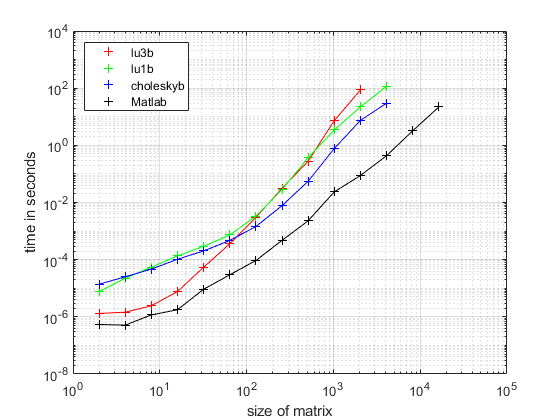
\includegraphics[scale = 1]{time.png}
\caption{Temps associé à la factorisation $\mathbf{LDL}^T$ (\textsc{Cholesky modifié}) en fonction des implémentations \texttt{lu} et la fonction \texttt{lu} de \textsc{Matlab}, en fonction de la taille de la matrice $\mathbf{A}$}
\end{figure}
On remarque que les coefficients directeurs des courbes est d'approximativement de $3$ pour chacun des algorithmes. Cependant, l'algorithme de \textsc{Cholesky} modifié est plus rapide pour des matrices suffisament grandes. Le facteur de gain est entre $2$ et $6$ mais n'est pas stable et la mesure est encore trop entachée d'erreurs. 

\subsection{Exercice 2 : Méthode de \textsc{Gauss} sur matrice tri-diagonale}

On cherche à factoriser une matrice tri-diagonale $\mathbf{A} = \mathbf{L} \mathbf{U}$ écrite comme :

\begin{equation*}\underbrace{
\begin{bmatrix}
a_1 & c_1^A & 0 & 0 & \cdots & 0 \\ 
b_1 & a_2 & c_2^A & 0 & \cdots & 0 \\
0 & b_2 & a_3 & c_3 & ~ & 0 \\
\vdots & ~ & \ddots & \ddots & \ddots & ~ \\
\vdots & ~ & ~ & \ddots & a_{n-1} & c_{n-1}^A \\ 
0 & ~ & ~ & ~ & b_{n-1} & a_n
\end{bmatrix}}_{\mathbf{A}} = \underbrace{\begin{bmatrix}
1 & 0 & 0 & 0 & \cdots & 0 \\ 
e_1 & 1 & 0 & 0 & \cdots & 0 \\
0 & e_2 & 1 &0 & ~ & 0 \\
\vdots & ~ & \ddots & \ddots & \ddots & ~ \\
\vdots & ~ & ~ & \ddots & 1 & 0 \\ 
0 & ~ & ~ & ~ & e_{n-1} &1
\end{bmatrix}}_{\mathbf{L}}.\underbrace{\begin{bmatrix}
d_1 & c_1 & 0 & 0 & \cdots & 0 \\ 
0 & d_2 & c_2 & 0 & \cdots & 0 \\
0 & 0 & d_3 & c_3 & ~ & 0 \\
\vdots & ~ & \ddots & \ddots & \ddots & ~ \\
\vdots & ~ & ~ & \ddots & d_{n-1} & c_{n-1} \\ 
0 & ~ & ~ & ~ & 0 & d_n
\end{bmatrix}}_{\mathbf{U}}
\end{equation*}
Soit, en calculant explicitement le produit $\mathbf{L} \mathbf{U}$ : 
\begin{equation*}
\begin{bmatrix}
a_1 & c_1^A & 0 & 0 & \cdots & 0 \\ 
b_1 & a_2 & c_2^A & 0 & \cdots & 0 \\
0 & b_2 & a_3 & c_3 & ~ & 0 \\
\vdots & ~ & \ddots & \ddots & \ddots & ~ \\
\vdots & ~ & ~ & \ddots & a_{n-1} & c_{n-1}^A \\ 
0 & ~ & ~ & ~ & b_{n-1} & a_n
\end{bmatrix} = \begin{bmatrix}
d_1 & c_1 & 0 & 0 & \cdots & 0 \\ 
d_1 e_1 & c_1 e_1 + d_2& c_2 & 0 & \cdots & 0 \\
0 & d_2 e_2 & c_2 e_2 + d_3 & c_3 & ~ & 0 \\
\vdots & ~ & \ddots & \ddots & \ddots & ~ \\
\vdots & ~ & ~ & \ddots & a_{n-1} & c_{n-1} \\ 
0 & ~ & ~ & ~ & d_{n-1} e_{n-1} & c_{n-1} e_{n-1} +d_n
\end{bmatrix}
\end{equation*}

Ainsi, il en découle le système suivant :

\begin{equation} \left\{
\begin{array}{ll}
c_{i}^A = c_i &\forall i \in [1, n-1] \\
a_1 = d_1 & \\
a_{i} = c_{i-1} e_{i-1} + d_i&\forall i \in [2, n]\\
b_i = d_i e_i&\forall i \in [1, n-1]\\
\end{array}
\right.
\end{equation}
sous certaines conditions, le système fournis :
\begin{equation} \left\{
\begin{array}{ll}
c_{i} = c_i^A &\forall i \in [1, n-1] \\
d_{i} = a_i - c_{i-1} e_{i-1} = a_i - \frac{c_{i-1} b_{i-1}}{d_{i-1}}&\forall i \in [2, n]\\
e_i = \frac{b_i}{d_i}&\forall i \in [1, n-1]\\
\end{array}
\right.
\end{equation}.

Cela aboutit à l'écriture de l'algorithme suivant :

\begin{algorithm}[H]
\caption{Factorisation LU pour matrice tridiagonale}\label{alg:two}
$c_1 = a_{1,2}$ \;
$d_1 = a_{1,1}$ \;
$e_1 = \frac{b_1}{d_1}$ \;
\For{$i \in [2, n-1]$}{
	$c_i = a_{i, i+1}$\;
	$d_{i} =  a_{i,i} - \frac{b_{i-1} c_{i-1}}{a_{i-1,i-1}}$ \;
	$e_{i} = \frac{b_i}{d_i}$ \;
}
$d_n =  a_{n,n} - \frac{b_{n-1} c_{n-1}}{a_{n-1,n-1}}$\;
\end{algorithm}

Il est bien-sur possible d'économiser de la place mémoire, comme expliqué ci-dessus pour la décomposition $\mathbf{L}\mathbf{D} \mathbf{L}^T$, avec un algorithme en place : 

\begin{algorithm}[H]
\caption{Factorisation LU en place pour matrice tridiagonale}\label{alg:two}
$a_{1,2} = a_{1,2}$ \;
$a_{2,1} = \frac{a_{2,1}}{a_{1,1}}$ \;
\For{$i \in [2, n-1]$}{
	$a_{i,i} =  a_{i,i} - \frac{a_{i, i-1} a_{i-1, i}}{a_{i-1,i-1}}$ \;
	$a_{i+1, i} = \frac{a_{i+1, i}}{a_{i,i}}$ \;
}
$a_{n,n} =  a_{n,n} - \frac{a_{n, n-1} a_{n-1, n}}{a_{n-1,n-1}}$\;
\end{algorithm}

\textit{Note : il faudra bien-sûr adapter les phases de résolution par montée et de descente pour admettre une matrice en-place.}

On remarque que la complexité asymptotique de la factorisation est $C_{tri} = \mathcal{O}(n)$, très loin de la complexité asymptotique de la factorisation dans le cadre de matrices pleines, qui est de $C_{full} = \mathcal{O}(n^3)$., De plus, l'empreinte mémoire asymptotique associée est $M_{tri} = \mathcal{O}(3n)$, contre $M_{full} = \mathcal{O}(n\times n)$. Il est alors absolument nécéssaire de privilégier les méthodes analogues lorsque les matrices possèdent des structures bandes. 

\textit{On rappelle que beaucoup de problèmes discrétisés peuvent s'écrire selon un problème bande. Cependant, il est parfois nécéssaire d'opérer des permutations afin de réduire au maximum la largeur de bande. Il faudrait alors étudier la complexité algorithmique du réindicage afin de déterminer dans quels cas le réindicage est à privilégier}

Voici une implementation sur \textsc{Matlab} de l'algorithme : 


\begin{figure}[H]
\begin{minipage}{0.5\textwidth}
\begin{lstlisting}[language=Matlab, caption=Factorisation LU de matrice trigonale]
function [L,U] = lutrig(A)
[n, n2] = size(A); 
L = eye(n,n);
U = zeros(n,n)
U(1,1) = A(1,1) ; 
L(2,1) = A(2,1) / A(1,1) ;
U(1,2) = A(1,2);
for i = [2:n-1]
    U(i,i+1)=A(i,i+1);
    U(i,i)=A(i,i)-A(i-1,i)*L(i,i-1);
    L(i+1,i)=A(i+1,i)/U(i,i);
end
U(n,n)=A(n,n)-A(n-1,n)*L(n,n-1);
end
\end{lstlisting}
\end{minipage}
\begin{minipage}{0.49\textwidth}
\begin{lstlisting}[language=Matlab, caption=Factorisation LU sur place de matrice trigonale]
function [A] = lutrigplace(A)
[n, n2] = size(A); 
 
 
A(1,1)=A(1,1) ; 
A(1,2)=A(1,2);
A(2,1)=A(2, 1)/A(1,1)
for i = [2:n-1]
    A(i,i+1)=A(i,i+1);
    A(i,i)=A(i,i)-A(i-1,i)*A(i,i-1);
    A(i+1,i)=A(i+1,i)/A(i,i);
end
A(n,n)=A(n,n)-A(n-1,n)*A(n,n-1);
end
\end{lstlisting}
\end{minipage}
\end{figure}

\begin{lstlisting}[language=Matlab, caption=Exemple de factorisation trigonale]
A
     5     4     0     0     0
     7     8     9     0     0
     0     3     2     7     0
     0     0     0     8     1
     0     0     0     3     2
L
    1.0000         0         0         0         0
    1.4000    1.0000         0         0         0
         0    1.2500    1.0000         0         0
         0         0         0    1.0000         0
         0         0         0    0.3750    1.0000
U
    5.0000    4.0000         0         0         0
         0    2.4000    9.0000         0         0
         0         0   -9.2500    7.0000         0
         0         0         0    8.0000    1.0000
         0         0         0         0    1.6250
L*U
     5     4     0     0     0
     7     8     9     0     0
     0     3     2     7     0
     0     0     0     8     1
     0     0     0     3     2
Factorisation en place
    5.0000    4.0000         0         0         0
    1.4000    2.4000    9.0000         0         0
         0    1.2500   -9.2500    7.0000         0
         0         0         0    8.0000    1.0000
         0         0         0    0.3750    1.6250
Difference A - L*U
     0
\end{lstlisting}


\subsection{Exercice 4 : Stockage CSR et CSC}
\textit{Note : CSR et CSC signifie Sparse Matrix Representation en ligne et en colonne.}

Soit la matrice creuse $\mathbf{A}$ suivante :

\begin{equation}\mathbf{A} = \begin{bmatrix}
15& 0& 0& 22 &0 &-15& 0& 0\\
0& 11& 3 &0 &0 &0 &2 &0\\
0 &0 &0& -6 &0 &0 &0 &0\\
0 &0 &0 &0 &0 &0& 0& 0\\
91& 0& 0& 0& 0& 0& 25& 7\\
0& 0& 28& 0& 0& 0& 0& -2
\end{bmatrix}
\end{equation}

Un stockage CSR peut être le suivant : 

\begin{figure}[H]
\centering
\begin{tabular}{|c|c|}
\hline
values		&   $\left[ 15, 22, -15, 11, 3, 2, -6, 91, 25, 7, 28, -2\right]$ \\ \hline
$p_x$ &  $\left[ 1, 1, 1, 2, 2, 2, 3, 5, 5, 5, 6, 6 \right]$  \\  \hline
$p_y$ &$\left[ 1, 4, 6, 2, 3, 7, 4, 1, 7, 8, 3, 8\right]$ \\  \hline
\end{tabular}
\caption{Stockage par coordonnées (COO)}
\end{figure}

\textit{Remarque : ce type de stockage peut aboutir à des couts supplémentaires lors de l'exécution de boucles de type \texttt{for j = [1:n]}. Cependant, cela a l'avantage de pouvoir stocker des nouvelles donnees à la suite des précédentes (dans le désordre).}

\begin{figure}[H]
\centering
\begin{tabular}{|c|c|}
\hline
values		&   $\left[ 15, 22, -15, 11, 3, 2, -6, 91, 25, 7, 28, -2\right]$ \\ \hline
$p$ &  $\left[ 1, 4, 6, 2, 3, 7, 4, 1, 7, 8, 3, 8\right]$  \\  \hline
$size$ &$\left[ 1, 4, 7,8 , 8, 11, 13\right]$ \\  \hline
\end{tabular}
\caption{Stockage compressé par ligne (CSR)}
\end{figure}

\begin{figure}[H]
\centering
\begin{tabular}{|c|c|}
\hline
values		&   $\left[ 15, 91, 11, 3, 28, 22, -6, -15, 2, 25, 7, -2\right]$ \\ \hline
$p$ &  $\left[ 1, 5, 2, 2, 6, 1, 3, 1, 2, 5, 5, 6 \right]$  \\  \hline
$size$ &$\left[ 1, 3, 4, 6, 8, 8, 9, 11, 13\right]$ \\  \hline
\end{tabular}
\caption{Stockage compressé par colonne (CSC)}
\end{figure}


%\begin{algorithm}[H]
%\caption{Transposition CR}\label{alg:two}
%\tcc{Initialisation of matrix}
%$s_{new} = zeros(size(M)(1))$ \;
%$p_{new} =  zeros(size(values))$ \;
%$n = 1$ \;
%\While{$n < size(M)(1)$}{
%	\tcc{for all possible lines}
%	\For{$i = [1:size(v)]$}{
%		\If{$p(i) = n$}{
%		\tcc{save the value}
%		}
%
%	}
%}
%\end{algorithm}


Une implémentation des algorithmes de conversion sont les suivants :
\begin{figure}[H]
\begin{minipage}{0.5\textwidth}
\begin{lstlisting}[language=Matlab, caption=Conversion vers le format POO]
function [values, px, py] = convert_poo(A)
[nx, ny] = size(A);
occ = 0 ;
for i = [1:nx]
    for j = [1:ny]
        if A(i,j) ~= 0 
            occ = occ + 1 ; 
        end
    end
end
values = zeros(occ, 1);
px = zeros(occ,1);
py = zeros(occ,1);
pos = 0
for i = [1:nx]
    for j = [1:ny]
        if A(i,j) ~= 0 
            pos = pos + 1 ;
            values(pos) = A(i,j) ; 
            px(pos) = i ;
            py(pos) = j ;
        end
    end
end


\end{lstlisting}
\end{minipage}
\begin{minipage}{0.49\textwidth}
\begin{lstlisting}[language=Matlab, caption=Conversion vers le format CSR]
function [values, p, s] = convert_csr(A)
[nx, ny] = size(A);
occ = 0 ;
for i = [1:nx]
    for j = [1:ny]
        if A(i,j) ~= 0 
            occ = occ + 1 ; 
        end
    end
end
values = zeros(occ,1) ; 
p = zeros(ny, 1);
s = zeros(nx+1, 1);  
pos = 0
size_s = 1 ; 
s(1) = size_s ; 
for i = [1:nx]
    for j = [1:ny]
        if (A(i,j) ~= 0)
            %% valeur non nulle 
            pos = pos + 1 ;
            size_s = size_s + 1 ; 
            values(pos) = A(i,j) ;
            p(pos) = j ; 
        end
    end
    s(i+1) =  size_s ;
end
\end{lstlisting}
\end{minipage}
\end{figure}
L'exécution de ces algorithmes sur la matrice $\mathbf{A}$ donne : 
\begin{lstlisting}[language=Matlab, caption=Résultat de conversion]
A
     5     0     0    22     0   -15     0     0
     0    11     3     0     0     0     2     0
     0     0     0    -6     0     0     0     0
     0     0     0     0     0     0     0     0
    91     0     0     0     0     0    25     7
     0     0    28     0     0     0     0    -2
values - POO
     5    22   -15    11     3     2    -6    91    25     7    28    -2
px - POO
     1     1     1     2     2     2     3     5     5     5     6     6
py - POO
     1     4     6     2     3     7     4     1     7     8     3     8
values - CSR
     5    22   -15    11     3     2    -6    91    25     7    28    -2
p - CSR
     1     4     6     2     3     7     4     1     7     8     3     8
s - CSR
     1     4     7     8     8    11    13
\end{lstlisting}
L'algorithme donne les mêmes résultats que la conversion théorique.

Un algorithme de produit matrice-vecteur est le suivant : 

\begin{lstlisting}[language=Matlab, caption=Algorithme de produit matrice CSR - vecteur]
function [v_r] = product_csr(v_a, p_a, s_a, v)
%% _a : for A matric
% v_ : values
% p_ : coordinates
% s_ : coordinate2    
[n1, n2] = size(s_a);
n1 = n1 - 1 ; 
v_r = zeros(n1, 0) ; 
index = 1
for i = [1:n1]
        sum = 0  ; 
        for j = [1 : s_a(i+1) - s_a(i)]
            sum = sum + v_a(s_a(i) + j - 1) * v(p_a(index)) ; 
            disp("ij")
            disp(v_a(s_a(i) + j - 1))
            disp(v(p_a(index)))
            index = index + 1 ; 
        end
        v_r(i) = sum ; 
end
\end{lstlisting}

\begin{lstlisting}[language=Matlab, caption=Résultats produit]
v
     1     2     3     4     5     6     7     8
A*v
    13    45   -24     0   322    68
product_csr(A_csr, p_csr, s_csr, v)
    13    45   -24     0   322    68
--------------------------------
v
     1     1     1     1     1     1     1     1
A*v
    22    16    -6     0   123    26
product_csr(A_csr, p_csr, s_csr, v)
    22    16    -6     0   123    26
--------------------------------
v
     1     0     0     1     0     0     1     0
A*v
    37     2    -6     0   116     0
product_csr(A_csr, p_csr, s_csr, v)
    37     2    -6     0   116     0
\end{lstlisting}

Les résultats sont bien-sûr cohérents avec les solutions analytiques.

La complexité du produit matrice vecteur pleines est pour les versions basiques de $C_{pleine} = \mathcal{O}(n\times m)$. Dans le cas d'utilisation de matrices creuses CSR, la complexité est $C_{CSR} \approx \mathcal{O}(size(v)$, avec $size(v)$ la taille du tableau des valeurs - qui représente le nombre de termes non nuls. On retrouve, bien-sûr,  $C_{CSR} = C_{pleine}$ lorsqu'il n'y a pas de valeurs non nulles dans la matrice. La gestion de la structure CSR génèrerait un surcoût par rapport au produit matriciel standard plein dans ce dernier cas - du fait de la lecture dans les tableaux \texttt{p} et \texttt{s} et les accès mémoires qui ne sont plus optimaux. Il existe cependant un taux de remplissage tel que les structures CSR seraient plus performantes que le produit naif.

\textit{Note : il est possible de concevoir un algorithme exploitant aussi un vecteur CSR.}












\section{Résolution de l'équation de la chaleur en 1D stationnaire}




Soit le modèle suivant : 
\begin{equation}
\left\{
\begin{array}{ll}
-k \frac{\partial^2 T }{\partial x^2 } &= g, ~~x \in ]0, 1[\\
T(0) &= T_0\\
T(1) &= T_1
\end{array}
\right.
\end{equation}

\subsection{Discrétisatiom du modèle continu}
En tant que fonction supposément suffisamment régulière, le développement de \textsc{Taylor} à l'ordre 2 fournis :
\begin{equation}
\left\{
\begin{array}{l}
T(x+h) = T(x) + h \frac{\partial T}{\partial x} + \frac{h^2}{2}\frac{\partial ^2 T}{\partial x^2} + o(h^2) \\ 
T(x-h) = T(x) - h \frac{\partial T}{\partial x} + \frac{h^2}{2}\frac{\partial ^2 T}{\partial x^2} + o(h^2) \\
\end{array}
\right.
\end{equation}

Ainsi, la somme et la soustraction des développements permet d'obtenir le schéma discrétisé suivant : 
\begin{equation}
\left\{
\begin{array}{l}
\left(\frac{\partial ^2 T}{\partial x^2}\right)_i = \frac{1}{h^2} \left( T_{i+1} + T_{i-1} - 2 T_i\right) ~~\forall x \in [1, n]\\
T(0) = T_0 \\
T(1) = T_1
\end{array}
\right.
\end{equation}
Il en résulte l'écriture matricielle ci-dessous. La prise en compte des conditions limites s'introduit dans le second membre.
Il en résulte le système suivant :

\begin{equation}
\underbrace{\begin{bmatrix}
2 & -1& 0 & 0 & \hdots&  \\
-1 & 2 &  1 & 0 & \hdots  &  \\
0&  \ddots&\ddots &\ddots && \vdots\\
\vdots& & \ddots&\ddots &\ddots &0 \\
&\hdots &0 & -1&2 & -1 \\
&\hdots &0 &0 &-1 & 2
\end{bmatrix}}_{\mathbf{A}} \underbrace{\begin{bmatrix}
U_1\\
U_2 \\
\vdots\\
\vdots\\
U_{n-1} \\
U_n 
\end{bmatrix}}_{U}=\underbrace{\begin{bmatrix}
\frac{h^2 g_1}{k}+T_0\\
\frac{h^2 g_2}{k}\\
\vdots\\
\vdots\\
\frac{h^2 g_{n-1}}{k} \\
\frac{h^2 g_n}{k} +T_1
\end{bmatrix}}_{f}
\end{equation}




\subsection{Méthode directe et stockage bande}

La résolution des formulations mathématiques par EDP discretisés nécéssite souvent la résolution d'un système linéaire de type $\mathbf{A} x = b$ tel que $\mathbf{A}$ est creuse, généralement bande suivant un réordonnancement des indices. 
Dans le cas de la chaleur 1D, la matrice $\mathbf{A}$ est de type tridiagonale. Afin de réduire le cout mémoire et la complexité calculatoire, il est possible de stocker uniquement les valeurs non nulles dans un tableau de valeurs. Il est proposé au sein du sujet d'adopter le stockage \textit{General Band}. En considérant $\mathbf{A}$ tridiagonale possédant $kl = ku = 1$ sur-diagonales et sous diagonales, le tableau de valeurs par bande $AB$ est de taille $n \times (kl + ku + 1) = 3 n$. Selon cette méthode, il y a alors une injection de l'espace de $A$ vers celui de $AB$ suivant $A_{i,j} = AB_{ku+1+i - j , j}$.

Soit l'exemple de la matrice tridiagonale du modèle :

\begin{equation}
\begin{pmatrix}
2 & -1& 0 & 0 & \hdots&  \\
-1 & 2 &  1 & 0 & \hdots  &  \\
0&  \ddots&\ddots &\ddots && \vdots\\
\vdots& & \ddots&\ddots &\ddots &0 \\
&\hdots &0 & -1&2 & -1 \\
&\hdots &0 &0 &-1 & 2
\end{pmatrix} \longrightarrow 
\begin{bmatrix}
\star & 2 & -1   \\
-1 & 2 &  -1 \\
-1 &  2 &-1  \\
\vdots&\vdots &\vdots\\
-1 & 2 & -1 \\
-1 & 2 & \star 
\end{bmatrix}
\end{equation}

\begin{equation*}
\longrightarrow 
\begin{Bmatrix}
\star & 2 & -1 &  -1 & 2 &  -1   & \hdots & -1  & 2 & \star \\
\end{Bmatrix}
\end{equation*}


Les bandes de valeurs de la matrice sont ordonnées selon les colonnes dans la matrice de stockage par bande. Autrement dit, la matrice bande selon les colonnes contient une succession de $-1$ selon sa première colonne et troisième colonne, et une succesion de $2$ selon la deuxième colonne. Puisque les bandes n'ont pas les mêmes longueurs, un offset est introduit tel quel la lecture horizontale des valeurs de la matrice bande corresponde à la lecture horizontale de la matrice initiale. Il apparait alors des positions représentées par $\star$ dont les valeurs n'importent pas. Le stockage en mémoire correspond au déroulement 1D de la matrice bande. Ainsi, la taille du tableau 1D de valeurs de la matrice $\A$ de taille $n\times n$ est $3 \times n$. 


\textit{Note : Il est parfois nécéssaire  d'allouer des espaces mémoires nécéssaires à la manipulation des données au sein des routines \texttt{dgbsv}. le tableau 1D contient alors $n$ valeurs initialement nulles.}

Le tableau 2D à bande par ligne est la transposée au tableau 2D à bande par colonnes. Le tableau 1D à bande par lignes est le déroulement selon les lignes du tableau 2D correspondant. Ainsi, les tableaux par lignes sont les suivants : 

\begin{equation}
\begin{pmatrix}
2 & -1& 0 & 0 & \hdots&  \\
-1 & 2 &  1 & 0 & \hdots  &  \\
0&  \ddots&\ddots &\ddots && \vdots\\
\vdots& & \ddots&\ddots &\ddots &0 \\
&\hdots &0 & -1&2 & -1 \\
&\hdots &0 &0 &-1 & 2
\end{pmatrix} \longrightarrow 
\begin{bmatrix}
\star & -1 & -1  & \hdots & -1 & -1  \\
2 & 2 & 2  & \hdots & 2 & 2  \\
-1 & -1 & -1  & \hdots & -1 & \star  \\
\end{bmatrix}
\end{equation}
\begin{equation*}
\longrightarrow 
\begin{Bmatrix}
\star & -1 & -1  & \hdots &  2 & 2   & \hdots & -1  & -1 & \star \\
\end{Bmatrix}
\end{equation*}

La fonction \texttt{malloc} permet d'allouer de la mémoire en \texttt{C}. L'allocation de la taille physique s'effectue par la multiplication de la taille de la donnée stockée par son occurence. Par exemple, l'allocation d'un tableau 1D en \texttt{C} de 8 \texttt{double} se fait suivant : 

\begin{lstlisting}[language=C, caption=Allocation tableau 1D]
double *tableau ; 
tableau = malloc( 8 * sizeof(double)) ; 
\end{lstlisting}

\texttt{tableau} est un pointeur. Ainsi, l'accès à la $i$-ème valeur s'effectue par \texttt{tableau[i]} ou par \texttt{\&tableau + i}.

\subsubsection{\texttt{DBGSV} et résolution de systèmes linéaires}


La méthode \texttt{DBGSV} fournis par \textbf{LAPACKE} permet de résoudre un système linéaire $\A x = b$ en utilisant l'écriture bande précédemment détaillée, en utilisant un principe de factorisation, puis de remontée/descente. Les valeurs sont stockées en double précision, sur 64 bits. Voici la syntaxte à utiliser pour son utilisation : 

\texttt{info =  LAPACKE\_dgbsv (matrix\_layout, n, kl, ku, nrhs, a, lda, ipiv, b, ldb);}

On utilise l'argument \textbf{LAPACK\_ROW\_MAJOR} et \textbf{LAPACK\_COL\_MAJOR} avec respectivement le stockage 1D des matrices bandes lignes et colonnes dévelopées ci-dessus. Le retour \texttt{info} permet de renvoyer un code d'erreur non-nul. La dimension principale souvent notée \texttt{ld} correspond à la dimenson principale, qui permet de retrouver le pas de déroulement lors du passage du tableau de valeurs 2D à bandes au tableau de valeurs 1D à bandes. Cela correspond alors à \texttt{lda = lab} en colonne et \texttt{lda = la} en lignes.

\subsection{Verification de \texttt{DGBSV}}

La résolution du système du problème selon les lignes et les colonnes fournis un code d'erreur \texttt{info} nul, ce qui est bon signe. Pour valider le vecteur solution obtenu par la résolution du système linéaire, le code initial suggère d'utiliser la formule d'erreur relative suivante :

\begin{equation}
	relres = \frac{\Vert x-\hat{x} \Vert}{\Vert \hat{x} \Vert}
\end{equation}

avec $x$ la solution obtenue par résolution et $\hat{x}$ la solution analytique. Les normes 2 et inf sont proposées afin d'analyser aussi l'erreur relative maximale.

Voici un tableau représentant les erreurs obtenues selon la taille, le type de norme. 

\textit{Note : les solutions $x$ obtenues selon l'algorithme en colonne et ligne sont identiques. Cela provient du fait que \texttt{dgbsv} effectue une transposée. L'ordre des calculs est ainsi stritement identique selon les deux variantes}.

\begin{figure}[H]
\centering
\begin{tabular}{|l|c|c|}
\hline
~ & $\Vert \Vert_2$ & $\Vert \Vert_{\infty}$ \\ \hline
$n = 50$  &$4.505236e-16$&$1.351527e-16$\\ \hline
$n = 500$&$1.548222e-14$&$2.793464e-15$\\ \hline
$n = 5000$&$1.759042e-12$&$2.737958e-13$\\ \hline
$n = 50000$&$6.380102e-11$&$1.231981e-11$\\ \hline
$n = 500000$&$8.533737e-08$&$1.409955e-08$\\ \hline
$n = 5000000$&$1.318371e-06$&$2.333718e-07$\\ \hline
\end{tabular}
\caption{Erreurs en fonction de la taille du problème}
\end{figure}

La méthode fournis alors des résultats satisfaisants pour des matrices de taille $n$ jusqu'a au moins 5 millions. Plus la matrice est grande, plus l'erreur relative est importante. Il existe une taille de matrice telle que la précision n'est plus acceptable. Il est alors nécéssaire soit de changer la méthode, soit d'utiliser une représentation des nombres plus précise.

Concernant le temps d'exécution, la variante en colonne est générallement légèrement plus rapide. 


\subsubsection{Méthode \texttt{DGBMV}}

La méthode \texttt{DGBMV} permet d'effectuer l'opération $y \leftarrow \beta y + \alpha \A x$. Elle s'appelle par CBLAS selon : 

\texttt{cblas\_dgbmv(cblas\_layout, cblas\_transa, m, n, ml, mu, alpha, a, lda, x, incx, beta, y, incy)}

\texttt{cblas\_layout} permet de fournir l'argument de stockage des matrices bandes en colonne ou en ligne. $a$, $x$ et $y$ correspondent aux pointeurs vers les tableaux de valeurs 1D.  \texttt{m} et \texttt{n} correspondent à la dimension des vecteurs $x$ et $y$. Voici comment a été utilisé la fonction en ligne et colonne : 


\begin{lstlisting}[language=C, caption=Utilisation de DGBMV]
ku = kl = 1 ; 
stride = 1 ; 
double alpha = ... ; 
double beta = ... ; 

cblas_dgbmv(CblasColMajor, CblasNoTrans, la, la, kl, ku, alpha, AB_col, lab, x_col, stride , beta, y_col,  stride); 

cblas_dgbmv(CblasRowMajor, CblasNoTrans, la, la, kl, ku, alpha, AB_row, lab, x_row, stride , beta, y_row,  stride);
\end{lstlisting}

La validation de l'utilisation et de l'implémentation de la méthode a été effectué suivant :
\begin{itemize}
\item execution avec $\beta$ non nul seulement ($\alpha = 0$) ;
\item produit matrice-vecteur avec un seul terme non nul ($\beta = 0$, $\alpha$ non nul). Le terme non nul est pris dans la matrice sur la bande inférieure à une position arbtraire. La position sur le vecteur $x$ coincide avec cette position afin de donner une case mémoire non nulle calculable ; 
\item produit matrice vecteur avec matrice identité ($\beta = 0$, $\alpha$ non nul) ;
\item test avec $\beta$ non nul, $\alpha$ non nul sur matrice identité.
\end{itemize}
Les résultats sont ensuite comparés aux valeurs analytiques. 

Voici le résultat  des tests sur différentes tailles de matrice  :

\begin{lstlisting}[language=C, caption=Vérification de l'implémentation de DGBMV]
Dimension : 8
--------- Exercice 4 - verification 1  ---------
Resultat  COL 1 OK
Resultat  ROW 1 OK

--------- Exercice 4 - verification 2  ---------
Valeur attendue : 47.416138
Resultat  COL 2 OK
Resultat  ROW 2 FAUX

--------- Exercice 4 - verification 3  ---------
Resultat  COL 3 OK
Resultat  ROW 3 FAUX

--------- Exercice 4 - verification 4  ---------
Resultat  COL 4 OK
Resultat  ROW 4 FAUX
--------------------------------------------------
Dimension : 800000

--------- Exercice 4 - verification 1  ---------
Resultat  COL 1 OK
Resultat  ROW 1 OK

--------- Exercice 4 - verification 2  ---------
Valeur attendue : 47.416138
Resultat  COL 2 OK
Resultat  ROW 2 FAUX

--------- Exercice 4 - verification 3  ---------
Resultat  COL 3 OK
Resultat  ROW 3 FAUX

--------- Exercice 4 - verification 4  ---------
Resultat  COL 4 OK
Resultat  ROW 4 FAUX
\end{lstlisting}

L'utilisation de \texttt{DGBMV} est correcte en colonnes mais éronnée en lignes. Suite a quelques tests, il semblerait que la méthode lignes lise la matrice dans un mauvais sens. L'utilisation de la transposition ne résoud rien.

\subsubsection{Factorisation LU pour matrice tridiagonale}

Les principes et une implémentation \textsc{Matlab} d'une factorisation LU pour matrice tridiagonale a déjà été présentée plus haut. L'implémentation en \texttt{C} utilise le même algorithme (non en-place). Une comparaison pourra alors être effectuée en comparant les valeurs obtenues en C et sur \texttt{Matlab}. On rappelle que l'algorithme a déjà été validé sur cette dernière plateforme. La différence ici est que la factorisation est efféctuée sur trois matrices bandes. Poir simplifier l'écriture, les matrices $\LL$ et $\U$ sont créées en mémoire sous forme de matrice bande tridiagonale, bien qu'une diagonale soit à valeurs nulles.

Voici une implémentation dans le cas de matrices bandes colonnes : 

\begin{lstlisting}[language=C, caption=Factorisation LU tridiagonale]
void LU_tri_col(double* A, double* L, double* U, int* la){
	// A est matrice bande triangulaire colonne
	// L et U reprennent alors le meme format 
	
	for (int i = 0 ; i < (*la) ; i ++){
		L[1 + i*3] = 1.0 ; 
	}	
	U[1] = A[1] ; 
	U[2] = A[2] ; 
	L[3] = A[3] / A[1] ; 
	for (int i = 1 ; i < (*la) - 1 ; i++){
		U[2 + 3 * i] = A[2 + 3 * i] ; 
		U[1 + 3 * i] = A[1 + 3 * i] - A[-1 + 3 * i]*L[3 * i] ; 
		L[3 + 3 * i] = A[3 + 3 * i]/U[1 + 3 * i] ; 
	}	 
	U[1 + 3 * ((*la) - 1 )] = A[1 + 3 * ((*la) - 1 )] - A[-1 + 3 * ((*la) - 1 )]*L[3 * ((*la) - 1 )] ;
\end{lstlisting}


Pour la matrice du problème avec $n=6$, l'algorithme fournit les matrices L et U suivantes : 

\begin{lstlisting}[language=C, caption=Factorisation LU tridiagonale]
L : 
0.000000        1.000000        0.000000
-0.500000       1.000000        0.000000
-0.666667       1.000000        0.000000
-0.750000       1.000000        0.000000
-0.800000       1.000000        0.000000
-0.833333       1.000000        0.000000

U :
0.000000        2.000000        -1.000000
0.000000        1.500000        -1.000000
0.000000        1.333333        -1.000000
0.000000        1.250000        -1.000000
0.000000        1.200000        -1.000000
0.000000        1.166667        0.000000
\end{lstlisting}

Les valeurs obtenues depuis \textsc{Matlab} sont similaires. L'algorithme est alors correctement implémenté. Les mesures d'erreur ne seront pas effectuées en C.

\subsection{Méthode de résolution itérative}

Les méthodes de résolution itératives offre la liberté de choisir un compromis temps d'exzcution / précision. A l'inverse des méthodes dites directes qui nécéssitent l'éxécution complète de l'algorithme pour obtenir un résultat exploitable, les approches dites itératives offrent la possibilité de consulter l'approximation de la solution au fil de l'exécution, offrant une meilleure flexibilité d'utilisation. De plus, elles exploitent souvent des opérations hautement parralélisables - comme le produit matrice vecteur - ce qui permet une meilleure scalabilité de la méthode par rapport aux approches directes. Il existe un large panel de methodes iteratives, des methodes elementaires de \textsc{Jacobi} aux approches de \textsc{Newton-Krylov}. Seules les premières seront étudiées.


\subsubsection{Etude des méthodes de \textsc{Jacobi} et \textsc{Gauss-Seidel}}

Soit le système linéaire $\A x = b, ~ \A \in \mathbb{R}^{n,n}$ à résoudre :
\begin{itemize}
\item $\D$ correspond à la matrice diagonale de $\A$ tel que $d_{i,i} = a_{i,i}, ~ d_{i,j} = 0~ \forall i \ne j$;
\item $\E$ correspond à une matrice triangulaire inférieure telle que $e_{i,j} = - a_{ij} \forall j < i$ et $e_{i,j} = 0$ sinon;
\item $\F$ correspond à une matrice triangulaire supérieure telle que $e_{i,j} = + a_{ij} \forall j > i$ et $e_{i,j} = 0$ sinon.
\end{itemize}
La méthode de \textsc{Jacobi} consiste en l'execution iterative su schema suivant :
\begin{equation}
x^{k+1} = x^k + \D^{-1} \left( b - \A x^k  \right)
\end{equation}
La méthode de \textsc{Gauss-Seidel} consiste en l'exécution itérative du schéma suivant : 

\begin{equation}
x^{k+1} = x^k + \left( \D - \E \right)^{-1} \left( b - \A x^k  \right)
\end{equation}
Les deux méthodes sont donc très similaires dans leurs implémentations. Une itération nécéssite le calcul d'une inverse - parfois triviale dans le cas de $\D^{-1}$ -, de deux produits matrices-vecteurs et d'une somme. La complexité de la somme est de $C^{\text{somme}} = \mathcal{O}(n)$. La complexité du produit matrice-vecteur est de $C^{\text{produit}} = \mathcal{O}(n^2)$.  La complexité algorithmique des deux algorithmes est alors de $C^{\text{J}} = \mathcal{O}(n + n^2)$ et $C^{\text{GS}} = \mathcal{O}(n + 2 \times n^2)$ pour un nombre d'itérations suffisamment grand - de sorte à povoir négliger le calcul de $\left( \D - \E \right)^{-1}$. La propriété de matrice creuse ou matrice bande peut aussi être exploitée afin de réduire la complexité algorithmique des produits matrice - vecteur, d'une complexité $C^{\text{produit}} = \mathcal{O}(n^2)$ vers une complexité $C^{\text{produit,bande}} \approx \mathcal{O}(3 \times n)$ dans le cas d'une matrice tridiagonale. Ainsi, les complexités associées aux schémas de \textsc{Jacobi} et de \textsc{Gauss-Seidel} sont de respectivement  $C^{\text{J,bande}} = \mathcal{O}(n + n + n + 3\times n) =\mathcal{O}(6\times n) $ et $C^{\text{GS,bande}} = \mathcal{O}(n + 3 \times n + n + 3\times n) =\mathcal{O}(8\times n) $. L'algorithme de \textsc{Gauss-Seidel}  impose plus de calculs mais converge plus rapidement \textbf{en général}.

\textbf{Exemple analytique de schéma :}

Soit la matrice tridiagonale suivante :
\begin{equation}
\A = \begin{bmatrix}
2 & -1 & 0  \\
-1 & 2 & -1  \\ 
0 & -1 & 2  \\ 
\end{bmatrix}
\end{equation}
Le vecteur solution initial $x^0$ est nul - arbitraire. Le vecteur terme source est considéré comme $b = \begin{bmatrix}
-5 & 0 & 5 \\
\end{bmatrix}^T$.

\textbf{Application de la méthode de \textsc{Jacobi} :}

\begin{equation}
x^1 = \begin{bmatrix}
0  \\
0 \\
0 \\
\end{bmatrix}+ \frac{1}{2} \left(\begin{bmatrix}
-5  \\
0 \\
+5 \\
\end{bmatrix} - \begin{bmatrix}
0  \\
0 \\
0 \\
\end{bmatrix}  \right) = \begin{bmatrix}
-2.5  \\
0 \\
+2.5 \\
\end{bmatrix}
\end{equation}

\begin{equation}
x^2 = \begin{bmatrix}
-2.5  \\
0 \\
+2.5 \\
\end{bmatrix}+ \frac{1}{2} \underbrace{ \left(\begin{bmatrix}
-5  \\
0 \\
+5 \\
\end{bmatrix} - \begin{bmatrix}
2 & -1 & 0  \\
-1 & 2 & -1  \\ 
0 & -1 & 2  \\ 
\end{bmatrix} \begin{bmatrix}
-2.5  \\
0 \\
+2.5 \\
\end{bmatrix}  \right)}_{\begin{bmatrix}
0 \\
0 \\
0
\end{bmatrix}} = \begin{bmatrix}
-2.5  \\
0 \\
+2.5 \\
\end{bmatrix}
\end{equation}


\textbf{Application de la méthode de \textsc{Gauss-Seidel} : }

\begin{equation}
\left( \D - \E \right)^{-1} = \begin{bmatrix}
2 & 0 & 0 \\ 
-1 & 2 & 0 \\ 
0  &  -1 & 2 
\end{bmatrix}^{-1} =  \begin{bmatrix}
1/2 & 0 & 0 \\ 
1/4 & 1/2 & 0 \\ 
1/8  &  1/4 & +1/2 
\end{bmatrix}
\end{equation}

\begin{equation}
x^1 = \begin{bmatrix}
0  \\
0 \\
0 \\
\end{bmatrix}+ \begin{bmatrix}
1/2 & 0 & 0 \\ 
1/4 & 1/2 & 0 \\ 
1/8  &  1/4 & 1/2 
\end{bmatrix} \left(\begin{bmatrix}
-5  \\
0 \\
+5 \\
\end{bmatrix} - \begin{bmatrix}
0  \\
0 \\
0 \\
\end{bmatrix}  \right) = \begin{bmatrix}
-5/2  \\
-5/4 \\
+15/8 \\
\end{bmatrix}
\end{equation}

\begin{equation}
x^2 = \begin{bmatrix}
-5/2  \\
-5/4 \\
+15/8 \\
\end{bmatrix}+ \begin{bmatrix}
1/2 & 0 & 0 \\ 
1/4 & 1/2 & 0 \\ 
1/8  &  1/4 & 1/2 
\end{bmatrix} \left(\begin{bmatrix}
-5  \\
0 \\
+5 \\
\end{bmatrix} - \begin{bmatrix}
-5/2  \\
-5/4 \\
+15/8 \\
\end{bmatrix}  \right) = \begin{bmatrix}
-3.125  \\
-0.625 \\
+2.187 \\
\end{bmatrix}
\end{equation}

\begin{equation}
x^2 = \begin{bmatrix}
-3.125  \\
-0.625 \\
+2.187 \\
\end{bmatrix}+ \begin{bmatrix}
1/2 & 0 & 0 \\ 
1/4 & 1/2 & 0 \\ 
1/8  &  1/4 & 1/2 
\end{bmatrix} \left(\begin{bmatrix}
-5  \\
0 \\
+5 \\
\end{bmatrix} - \begin{bmatrix}
-3.125  \\
-0.625 \\
+2.187 \\
\end{bmatrix}  \right) = \begin{bmatrix}
 -2.8125 \\
   -0.3125 \\ 
    +2.3438\\
\end{bmatrix}
\end{equation}


La méthode de \textsc{Jacobi} converge dans cet exemple vers la solution analytique en une itération. Cela est un cas très particulier et n'est pas général. La methode de \textsc{Gauss-Seidel} semble converger vers la solution analytique. La matrice $\left( \D - \E \right)^{-1}$ est la même pour chaque itération. Il est alors possible de la calculer une seule fois. 


Ces méthodes ont été implémentées sur \textsc{Matlab} selon deux variantes "boucle" et "matriciel". Voici les implémentations matricielles des méthodes avec prise en compte de la sous-relaxation : 


\begin{figure}[H]
\begin{minipage}{0.5\textwidth}
\begin{lstlisting}[language=Matlab, caption=Jacobi]
function [x] = jacobim(Dinv, N, b, x, w, iteration)
% Dinv est la valeur diagonale inverse de A
% N est N = A - D(A), soit A prive de sa diagonale
% b est le second membre
% xinit est le vecteur solution a l'etat initial
% iteration est le nombre d'iterations du schema iteratif
% sortie : x est le vecteur solution
[n,n1] = size(b) ;
for it = [1 : iteration]
    x = w * Dinv * ( N * x + b) + (1 - w) * x ;  
end
end
\end{lstlisting}
\end{minipage}
\begin{minipage}{0.499\textwidth}
\begin{lstlisting}[language=Matlab, caption=Gauss-Seidel]
function [x] = gauss_seidelm(Pinv, N, b , x, w, iteration)
% A est la matrice du probleme



% b est le second membre
% xinit est le vecteur solution a l'etat initial
% iteration est le nombre d'iterations du schema iteratif
% sortie : x est le vecteur solution
[n,n1] = size(b) ;
for it = [1 : iteration]
    x = w * Pinv * ( N * x + b) + (1 - w) * x ; 
end
end
\end{lstlisting}
\end{minipage}
\end{figure}
Les algorithmes ont été executés sur le probleme de \textsc{Poisson} 1D et l'erreur relative a été calculée en fonction de plusieurs paramètres ; 
\begin{itemize}
\item le long des itérations, jusqu'à $10^4$ itérations ;
\item la taille du problème, de 22 à 800;
\item le coefficient $w$ de sous-relaxation, entre $w \in [0, 1]$;
\item selon les méthodes de \textsc{Jacobi} et de \textsc{Gauss-Seidel}.
\end{itemize}

L'erreur relative est calculée avec les normes $\Vert \Vert_2$ telles que $e = \frac{\Vert x - \hat{x} \Vert_2}{\Vert \hat{x} \Vert_2}$. Les prochaines observations sont similaires en norme infinie.

Voici le tracé des faisceaux d'erreurs relatives selon $w$ constant ($w = 1$), puis selon $n$ constant ($n$ = 800) : 

\begin{figure}[H]
\begin{minipage}{0.5\textwidth}
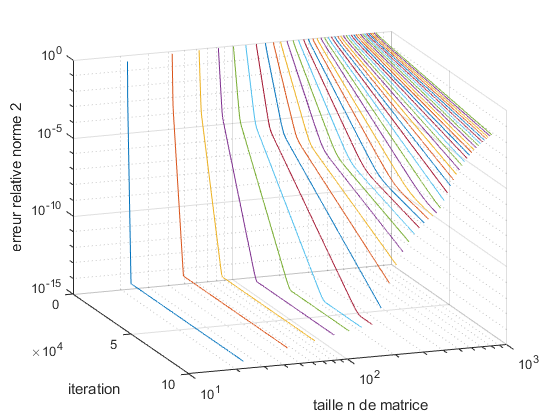
\includegraphics[scale = 0.63]{j_i_n_2.png}
\caption{\textsc{Jacobi}}
\end{minipage}
\begin{minipage}{0.499\textwidth}
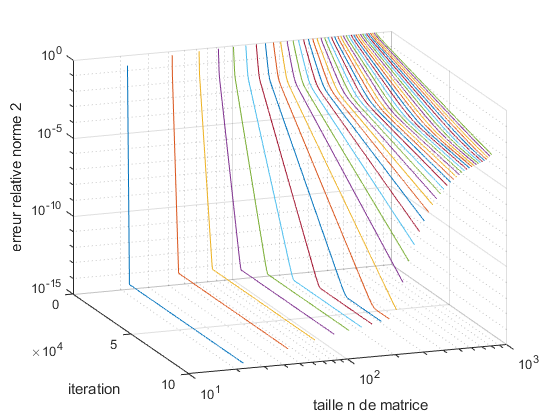
\includegraphics[scale = 0.63]{gs_i_n_2.png}
\caption{ \textsc{Gauss-Seidel}}
\end{minipage}
\caption{Convergence des méthodes  ($w = 1$)}
\end{figure}

\begin{figure}[H]
\begin{minipage}{0.5\textwidth}
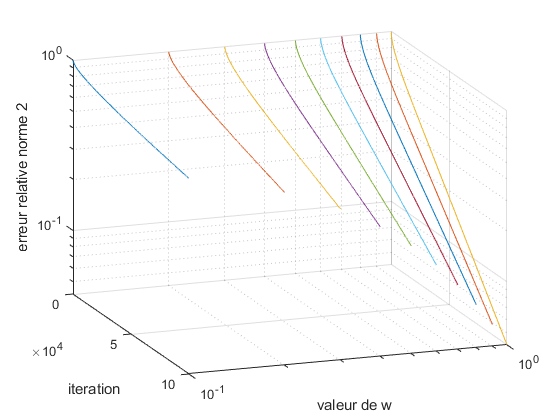
\includegraphics[scale = 0.63]{j_i_w_2.png}
\caption{\textsc{Jacobi}}
\end{minipage}
\begin{minipage}{0.499\textwidth}
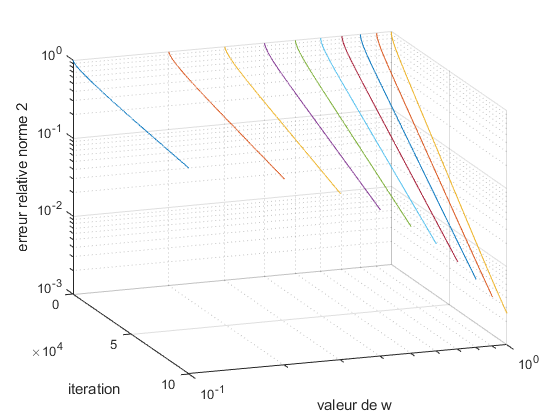
\includegraphics[scale = 0.63]{gs_i_w_2.png}
\caption{ \textsc{Gauss-Seidel}}
\end{minipage}
\caption{Convergence des méthodes ($n = 800$)}
\end{figure}

Le tracé des fasceaux de comvergence permet d'effectuer les observations suivantes :

\begin{itemize}
\item Les deux méthodes convergent vers la solution analytique dans tous les cas (la faible vitesse d'execution ne permet pas de le valider explicitement sur ces faisceaux de courbes sur des très grandes matrices). Les résidus à convergence avoisinent la précision limite $10^{-15}$ ; 
\item Plus le nombre de degrès de liberté du problème de \textsc{Poisson} est élevé, moins la convergence est rapide. D'ailleurs, c'est la raison pour laquelle il est utile de s'intéresser aux méthodes multigrid ou de décomposition de domaines (exemple : approche \textsc{LATIN}) qui permet de résoudre plusieurs petits problèmes, permettant d'accélérer la convergence globale de la méthode ;
\item La convergence est plus rapide pour $w=1.0$ lorsque $n = 800$. Attention : cela ne semble pas être le cas pour des problèmes plus petits ;
\item La vitesse de convergence est constante par morceaux - il semblerait que la vitesse de convergence soit réduire d'un facteur 2 en echêlle logarithmique d'un segment à l'autre; 
\item la méthode de \textsc{Gauss-Seidel} converge approximativement deux fois plus rapidement que la méthode de \textsc{Jacobi}. Cette observation n'est pas exacte car dépend légèrement de la taille du problème. Le facteur 2 sur la vitesse de convergence peut d'ailleurs être expliquée par la propriété $\rho\left( \B_{GS}\right) = \left(\rho\left( \B_{J}\right)\right)^2$. La méthode de \textsc{Jacobi} est cependant plus rapide à calculer et il faudra privilégier la méthode en fonction de la capacité personnelle à l'optimiser.
\end{itemize}
\subsubsection{Etude du processus iteratif de \textsc{Richardson}}

Soit le processus itératif de \textsc{Richardson} tel que : 

\begin{equation}
x^{k+1} = x^{k} +   \alpha \left( b - \A x^k\right)
\end{equation}
Par identification directe, il est possible d'ecrire ce schema selon la matrice d'iteration $G_{\alpha}$ : 
\begin{equation}
x^{k+1} = \underbrace{\left( I_n - \alpha \A \right)}_{\G_{\alpha}}x^k + \alpha b
\end{equation}

Soit les i valeurs et vecteurs propres $\lambda_{\A}^i$, $u_{\A}^i$ de $\A$ possiblement multiples. Ainsi, $\forall i \in [\![ 1, Dim(\A)]\!], ~ \A u^i_{\A} = \lambda_{\A} u_{\A}^i$. Les valeurs propres de $I_n$ sont toutes unitaires en tant que matrice identité. Ainsi, en considérant les valeurs et vecteurs propres de $\G_{\alpha}$, i.e. $\forall i \in [\![ 1, Dim(\G)]\!], ~ \G u^i_{\G} = \lambda_{\G} u_{\G}^i$, on remarque que :

\begin{equation}
\alpha \A u^i_{\A} =\alpha \lambda_{\A} u_{\A}^i \Longrightarrow  \underbrace{\left(-\alpha \A + I_n \right)}_{\G_{\alpha}} u^i_{\A} = \underbrace{\left(- \alpha \lambda_{\A}  + 1 \right)}_{\lambda_{\G}^i} u_{\A}^i
\end{equation}
Ainsi, la base de vecteurs propres de $\A$ et $\G_{\alpha}$ sont les mêmes. Les valeurs propres associées suivent $\lambda_{\G}^i = 1 -\alpha \lambda_{\A}^i$. Ainsi, les valeurs propres de $\G_{\alpha}$  sont telles que : 
\begin{equation}
\lambda_{\G}^i \in \left[ \underbrace{\alpha~ min\left( 1 - \lambda_{\A}^i \right)_{i}}_{\lambda_{\G}^{\text{min}}}  , \underbrace{\alpha~ max\left(1 - \lambda_{\A}^i \right)_{i}}_{\lambda_{\G}^{\text{max}}}\right]
\end{equation}

La methode associée au processus de \textsc{Richardson} converge si et seulement si $\max{\left(\vert \lambda_{\G}^i \vert\right)} < 1$ (condition sur le rayon spectral de la matrice d'itération). Ainsi, la condition de convergence s'établit par : 

\begin{equation}
\vert 1 - \alpha \lambda_{\A}^i \vert < 1 ~ \forall i \in [\![ 1, n]\!] \Longleftrightarrow \lambda_{\A}^i \in \left] 0 , \frac{2}{\alpha}\right[~ \forall i \in [\![ 1, n]\!]
\end{equation}

La convergence du processus dépend alors de la valeur de $\alpha$, ou à $\alpha$ fixé, des valeurs propres de $\A$. On peut néanmoins déterminer $\alpha_{m}$ minimisant le rayon spectral de la matrice d'itération, permettant d'améliorer les bornes de convergence du schéma itératif : 

\begin{align}
\text{Trouver } \alpha_m \text{ tel que } \vert 1 - \alpha_m \lambda_{\A}^i \vert \text{ minimal } \Longrightarrow &
\left( 1 - \alpha_m \lambda_{\A}^{\text{min}}\right) = - \left( 1 - \alpha_m \lambda_{\A}^{\text{max}}\right)  \\
\Longrightarrow& ~ \alpha_m = \frac{2}{\lambda_{A}^{\text{min}} + \lambda_{A}^{\text{max}}} 
\end{align}


La méthode s'implémente facilement sous \textsc{Matlab} et \textsc{Scilab} suivant : 
\begin{lstlisting}[language=Matlab, caption=Richardson]
function [x] = richardson(Pinv, N, b , x, w, iteration)
%% Pinv est la matrice de preconditionnement
%% A est la matrice du probleme
%% b est le second membre
%% x est le vecteur solution a l'etat initial
%% iteration est le nombre d'iterations du schema iteratif
%% sortie : x est le vecteur solution
[n,n1] = size(b) ;
for it = [1 : iteration]
    x = x + alpha * Pinv * (b - A * x) ; 
end
\end{lstlisting}


Une étude de convergence a été effectuée en fonction de $\alpha$ sur le problème de \textsc{Poisson} 1D selon une taille $n = 10$ et une taille $n = 1000$. Les valeurs de $\alpha$ sont au nombre de 100 entre 0 et 1. 100 itérations pour le premier problème et 1000 itérations sur le second problème ont ete efféctués. Les valeurs $\alpha$ tels que l'erreur relative est inférieure à 1 sont enregistrées (les schémas qui divergent retournent une erreur infinie).  Voici les intervalles contenant la valeur limite $\alpha_{lim}$ de convergence :

\begin{figure}[H]
\centering
\begin{tabular}{|c|c|c|}
\hline
&&\\
~ & $a_{lim}$& $\frac{2}{\rho(\A)}$ \\ 
&&\\\hline
$n = 10$  & $[0.510 , 0.511] $ &$0.5103$\\ \hline
$n=100$ & $[0.500 , 0.501]$ & $0.5001$\\ \hline
\end{tabular}
\end{figure}

Ainsi, le schéma semble diverger conformment à la limite analytique $a_{lim}$. On note que le rayon spectral de $\A$ dépend de la dimension $n$ du problème.

Voici les erreurs de la méthoe pour $n = 100$ en fonction de $alpha \in [0 , a_{lim}]$ : 




\begin{figure}[H]
\begin{minipage}{0.5\textwidth}
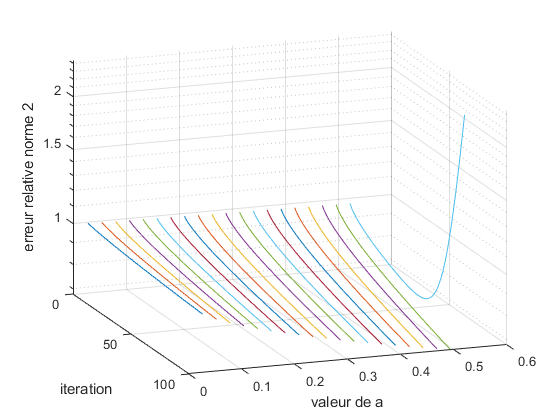
\includegraphics[scale = 0.63]{j_i_a_2_100.png}
\caption{\textsc{Richardson}, $100$ itérations}
\end{minipage}
\begin{minipage}{0.499\textwidth}
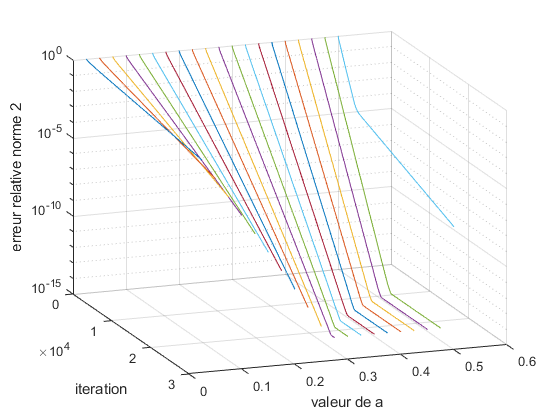
\includegraphics[scale = 0.63]{j_i_a_2_30000.png}
\caption{ \textsc{Richardson}, $30000$ itérations }
\end{minipage}
\caption{Convergence des méthodes  ($n = 100$)}
\end{figure}


La première figure propose l'évolution de l'erreur relative pour un $\alpha$ divergent qui n'apparait pas sur la seconde figure. Grossièrement, plus la valeur de $\alpha$ est proche de $\alpha_{lim}$, plus la convergence est rapide.  Cependant, il existe une valeur très proche de $\alpha_{lim}$, à savoir $\alpha =  0.51005$ pour $\alpha_{lim} = 0.5001$ tel que la convergence est perturbée, probablemet du fait de la précision utilisée. Par prudence, il est préférable d'utiliser une valeur suffisamment éloignée pour gagner en robustesse. L'utilisation de la valeur $\alpha = \frac{1}{2}$, qui correspond d'ailleurs à la méthode de \textsc{Jacobi}, convient parfaitement pour la résolution du problème.

\section{Conclusion}

Il est possible d'exploiter le caractère creux des matrices de certains problèmes physiques à résoudre en utilisant des structures de type CSR ou bandes. Cela permet, notamment, de réduire la complexité en mémoire des résolutions, mais aussi la complexité algorithmique des algorithmes tels que le produit matrice/vecteur, très utiles dans le cadre de la résolution de systèmes linéaires itératives. Ces dernières permettent d'approximer une solution avec un moindre coût par rapport aux méthodes itératives. De simples équations mathématiques permettent de déterminer notamment que la méthode de \textsc{Gauss-Seidel} converge plus rapidement que la méthode de \textsc{Jacobi}, ou qu'il existe dans \textsc{Richardson} des valeurs des paramètre $\alpha$ assurant stabilité ou optimalité de la convergence. Cependant, les méthodes de \textsc{Jacobi} et de \textsc{Richardson} sont plus faciles à implémenter et à optimiser. Il est alors important d'étudier et de concevoir des méthodes itératives, et les algorithmes en général en prenant aussi en compte le critère d'optimisation informatique.\\
D'autres méthodes permettant d'accélérer la résolution de certains problèmes existent, comme les \textit{méthodes de préconditionnement} - surtout lorsque le conditionnement du problème est mauvais - mauvais conditionnement qui d'ailleurs peut ralentir la convergence - , les \textit{méthodes de \textsc{Krylov}} ou \textit{GMRES}, très efficaces sur GPU notamment, et les \textit{approches de décomposition de domaines} qui trouvent leurs utilités sur des problèmes en très grandes dimensions.


\end{document}